\subsection{Модель генерации кластеров}
На стадии разработки алгоритма для проверки способности выбранного подхода выделять кластеры и отсекать неинформативные признаки была разработана модель генерации многомерных объектов по многомерному нормальному распределению. Такой подход при генерации позволяет задать форму кластера как многомерный эллипсоид, а возможность задавать корреляции между признаками позволяет заложить в модель число заранее известных нерепрезентативных признаков, на которых можно проверить работу алгоритмов обзора.

Для реализации n-мерной нормально распределенной случайной величины с заданной матрицей ковариации применялся следующий алгоритм:
\begin{enumerate}
  \item Реализация n случайных нормально распределенных величин, соответствующих каждой компоненте n-мерного пространства
  \item Формирование матрицы нескореллированных признаков $X$
  \item Вычисление матрицы преобразования $A$ из условия $AA^T=\text{Cov}$
  \item Вычисление скореллированых признаков $Y=AX$
\end{enumerate}

\begin{figure}[H]
	\center
  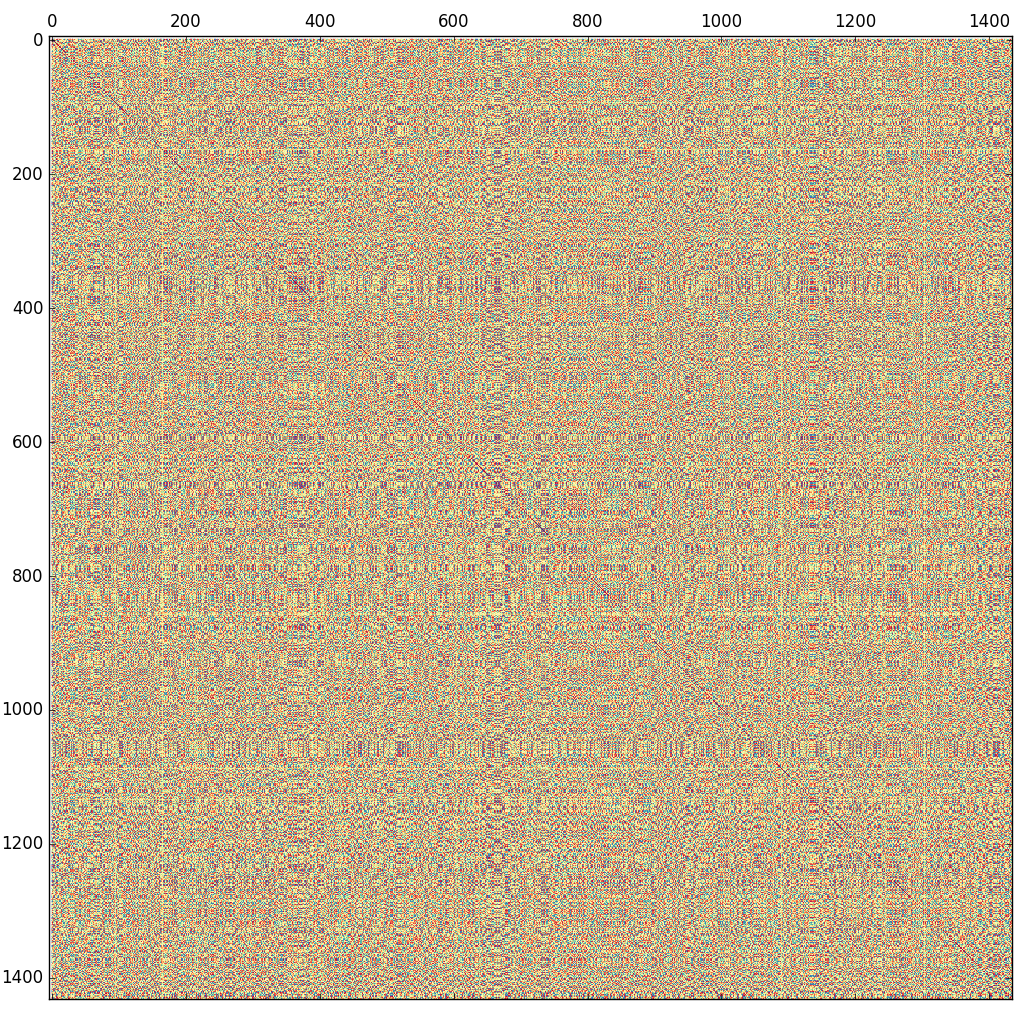
\includegraphics[width=0.5\linewidth]{pics/correlations_blob.png}
  \caption{Карта матрицы корреляций исходных признаков. Красный обозначает корреляцию 1, синий -- -1.}
  \label{correlation_blob}
\end{figure}

\begin{figure}[H]
	\center
  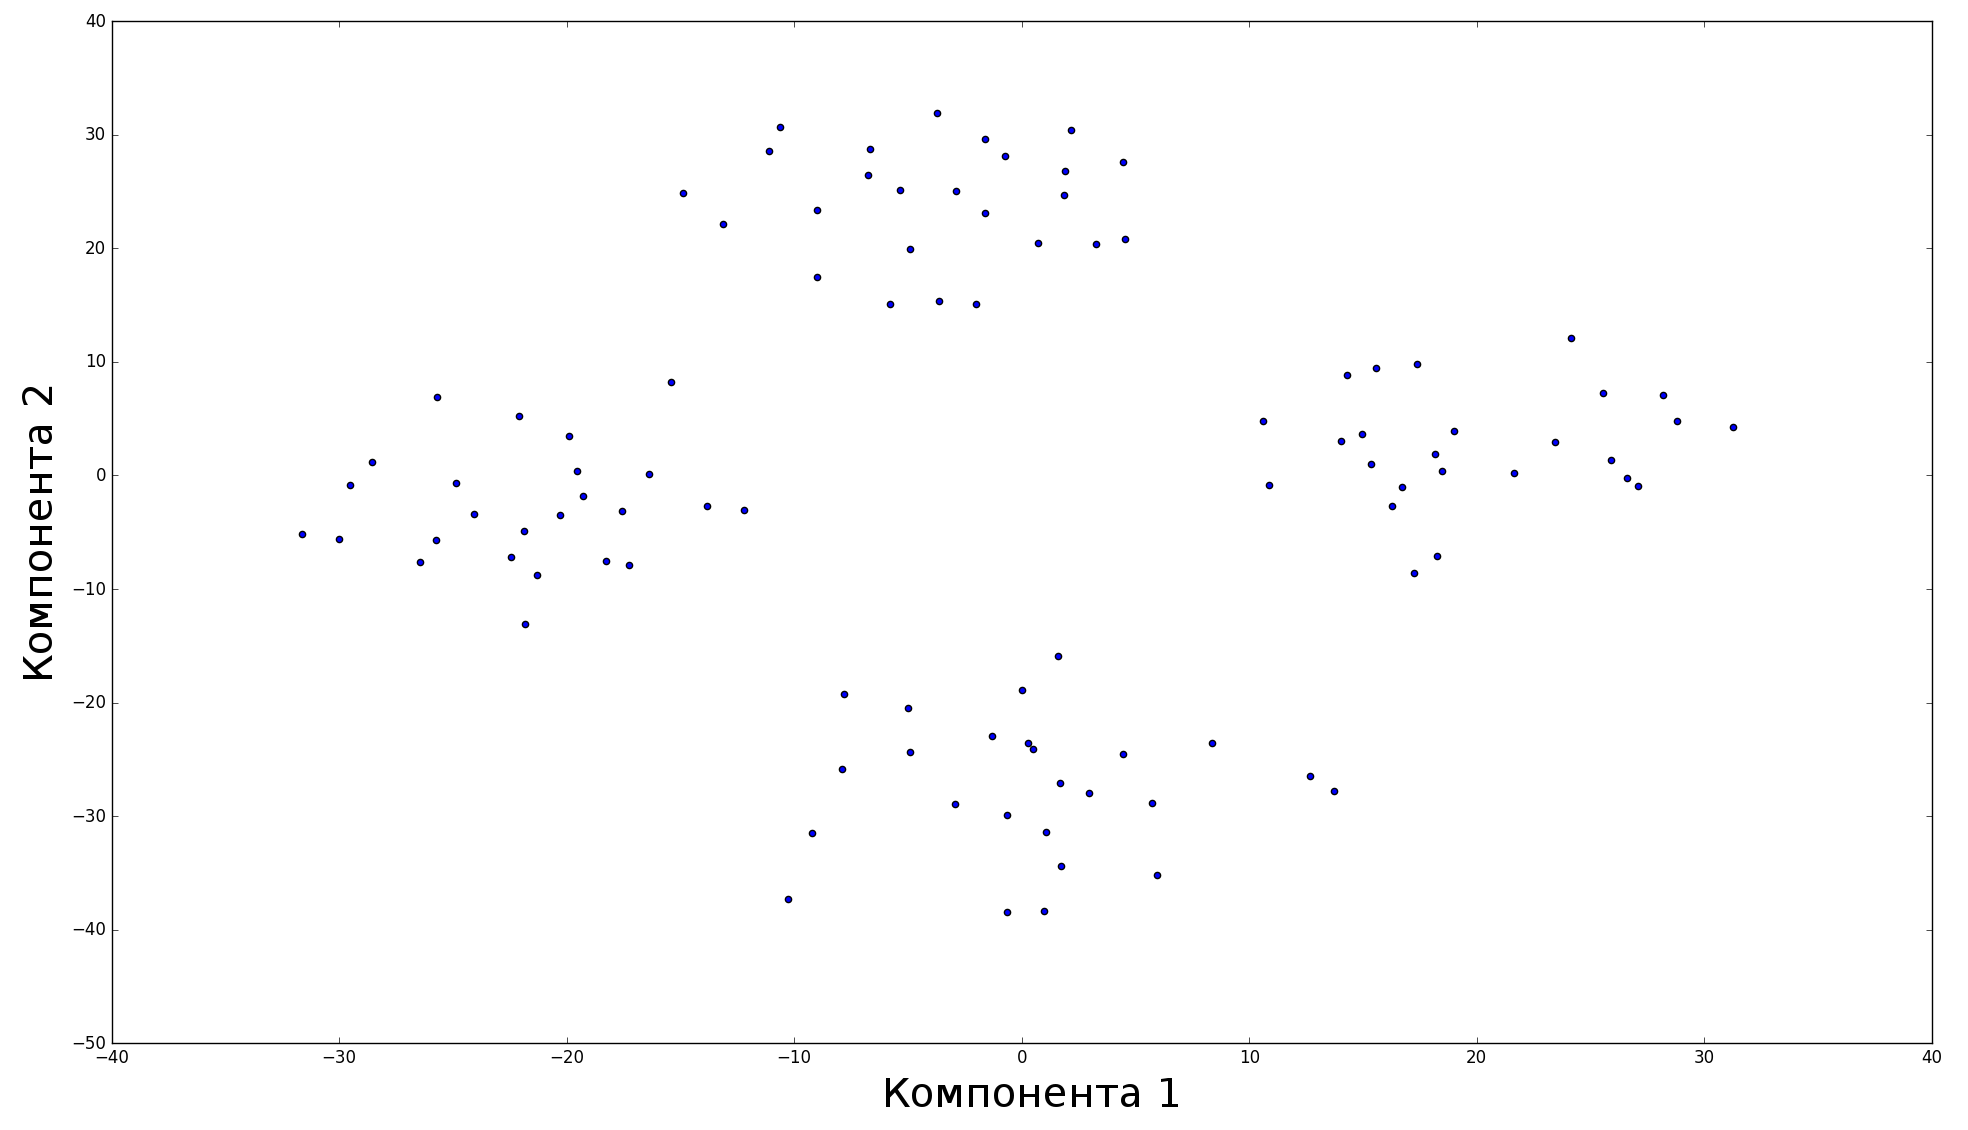
\includegraphics[width=\linewidth]{pics/tsne_blob.png}
  \caption{Визуализация смоделированных данных методом t-SNE}
  \label{tsne_blob}
\end{figure}

Для оценки работы алгоритмов был сгенерирован набор многомерных данных, включающий 100 объектов с 1500 признаками, из которых 100 признаков генерировались независимо, то есть считались важными в рамках данной модели, а 1400 генерировались как комбинации окажных признаков. Так же был на основе сгенерированного набора данных был построен стандартизированный набор данных, установивший матожидание каждого признака равным 0, а дисперсию равной 1.

\subsection{Разработка алгоритмов кластеризации}
Для реализации алгоритмов кластеризации были отобраны алгоритмы аггломеративной иерахической и спектральной кластеризации. Для иерархической кластеризацираци выбрано расстояние Уорда,лучше остальных альтернатив разделяющее кластеры, как критерий для объединения кластеров, и евклидова метрика как расстояние между отдельными объектами. В спектральной кластеризации применялась нормировка лапласиана средним арифметическим.

\begin{figure}[H]
	\center
  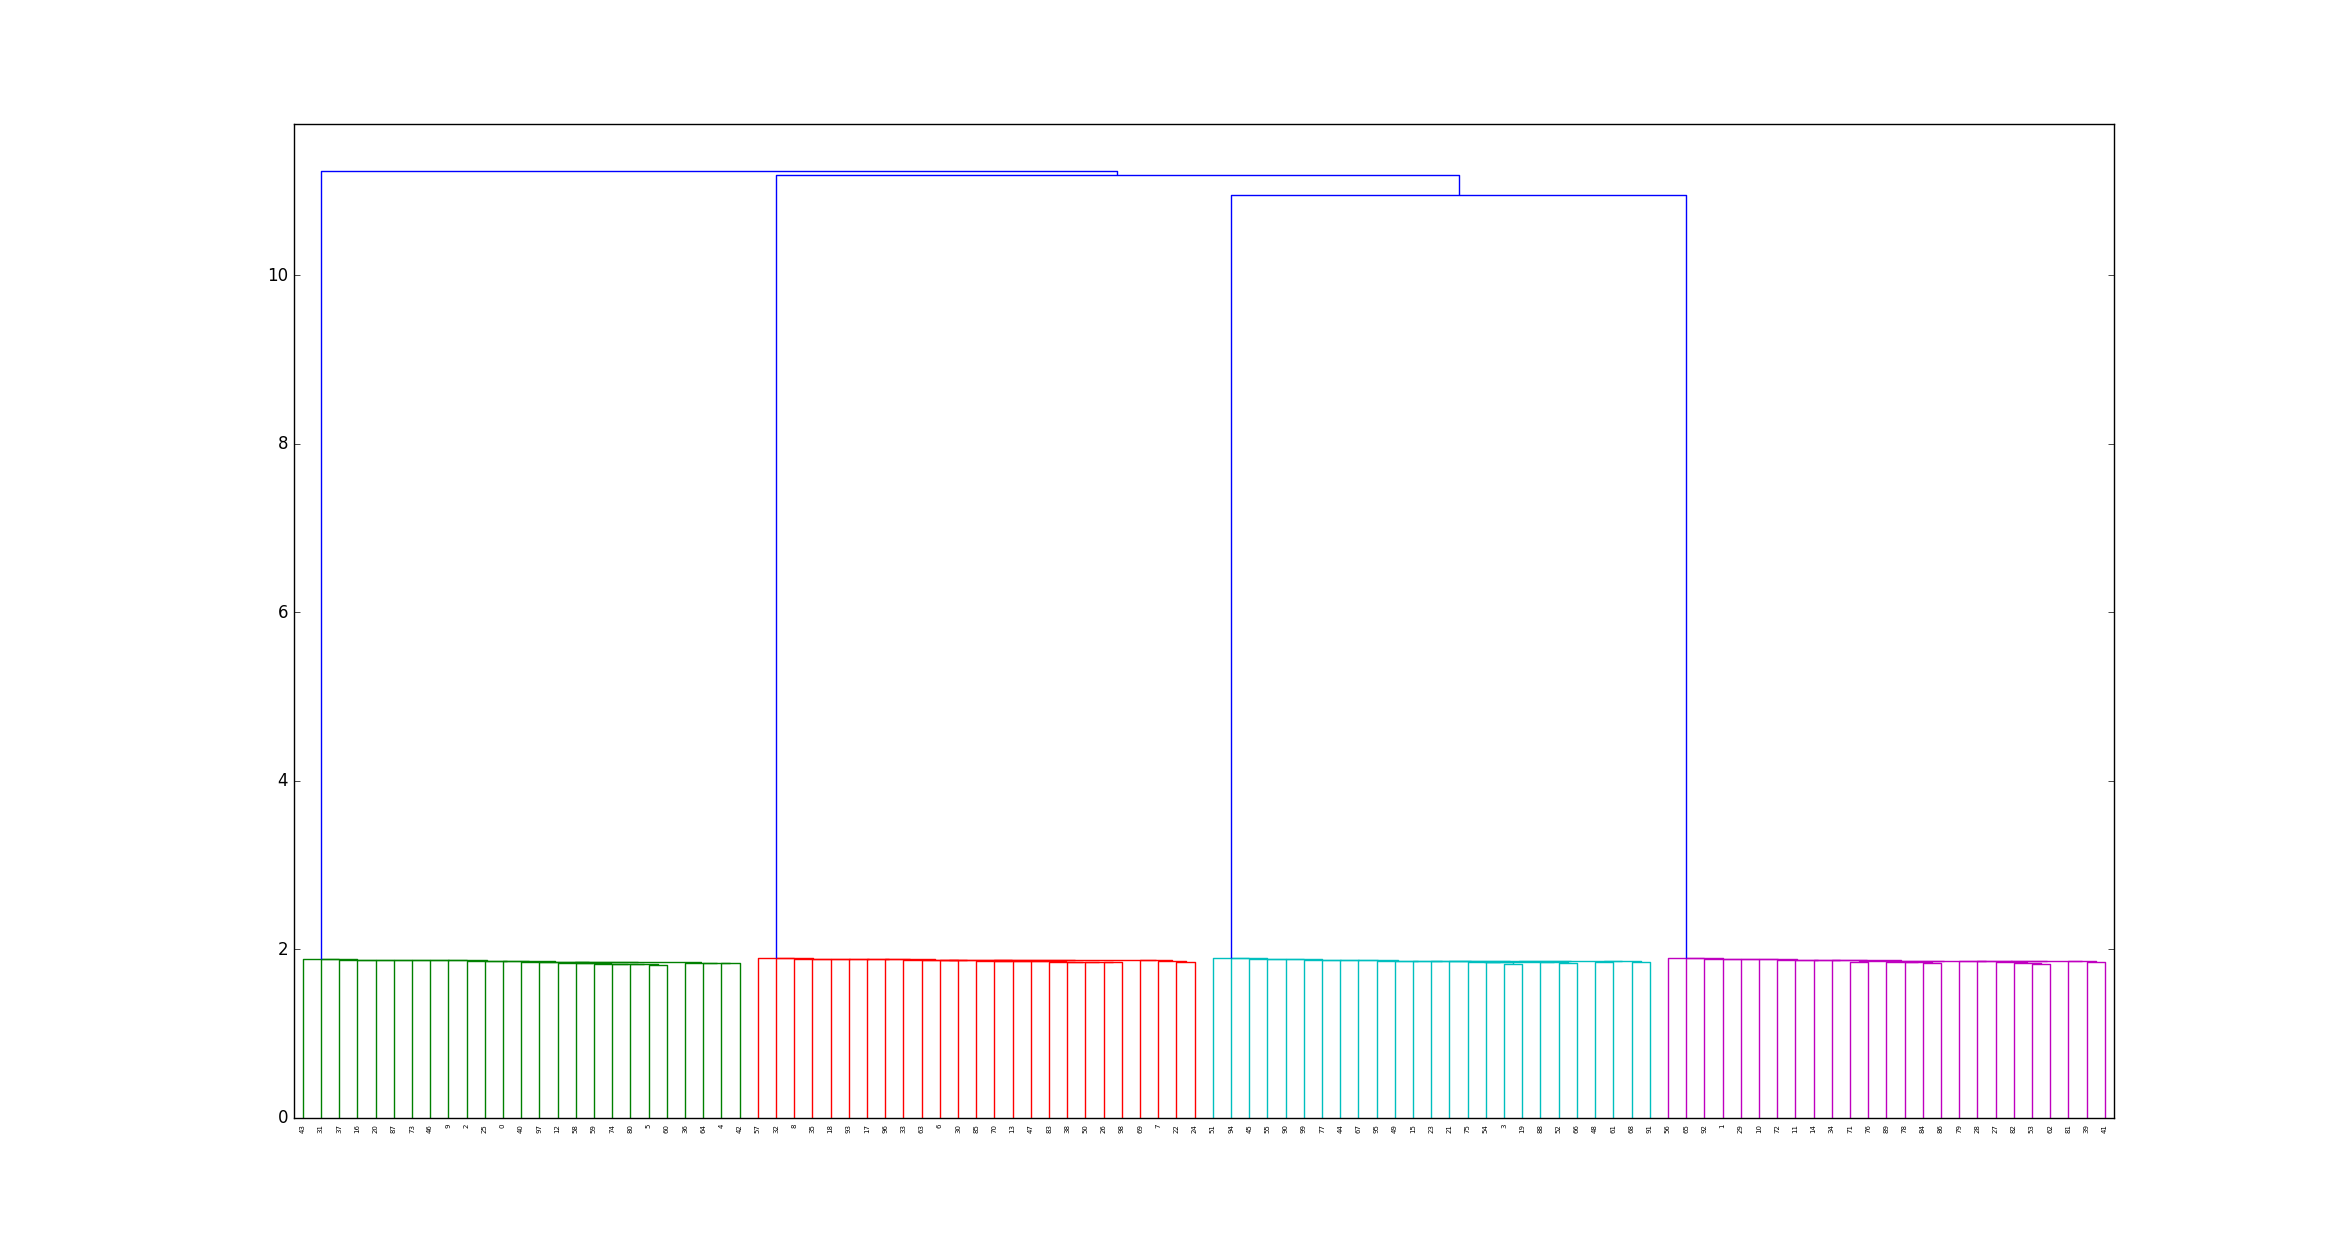
\includegraphics[width=\linewidth]{pics/dendrogram_blob.png}
  \caption{Результат иерархической кластеризации смоделированных данных}
  \label{dendrogram_blob}
\end{figure}

Как видно из дендрограммы, иерархическая кластеризация хорошо разделяет кластеры в смоделированных данных. 

\subsection{Разработка алгоритмов отбора признаков}
\subsubsection{Вычисление важности признаков из спектра лапласиана графа}
Как было отмечено ранее, алгоритмы отбора признаков состоят из базовой части вычисления спектра лапласиана графа ближайших соседей и дополнительных действий, разных для каждого алгоритма. Ниже мы рассмотрим действие каждого из этих факторов. 
\subsubsection{Применение ядер к функции ранжирования}
SPEC характеризуется применением различных неотрицательных функций для преобразования лапласиана. Такие трансформации способствуют лучшей отделяемости кластеров друг от друга. Для данной задачи в качестве ядра была выбрана степенная функция $\gamma(r) = r^2$, показывающая лучшее отделение кластеров в задаче разделения групп новостей. 
\begin{figure}[h]
  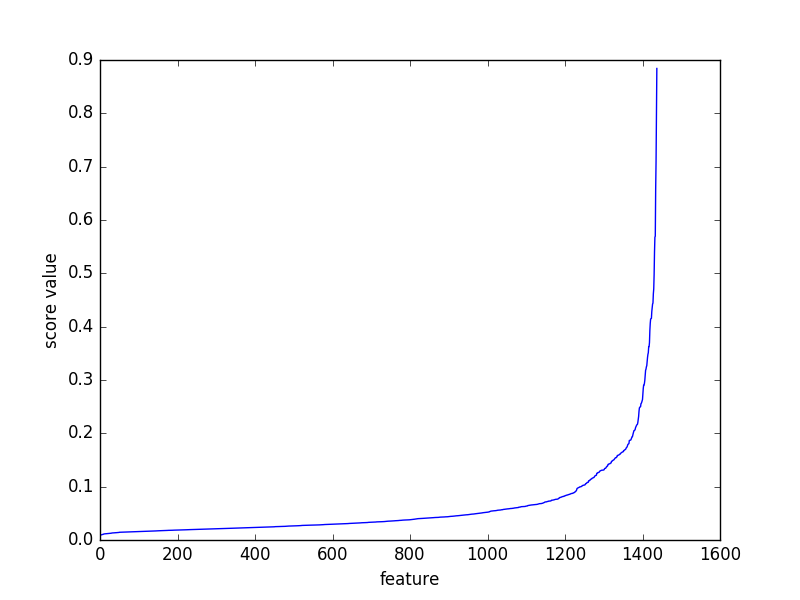
\includegraphics[width=0.5\linewidth]{pics/lp_unnorm_euclidean.png}
  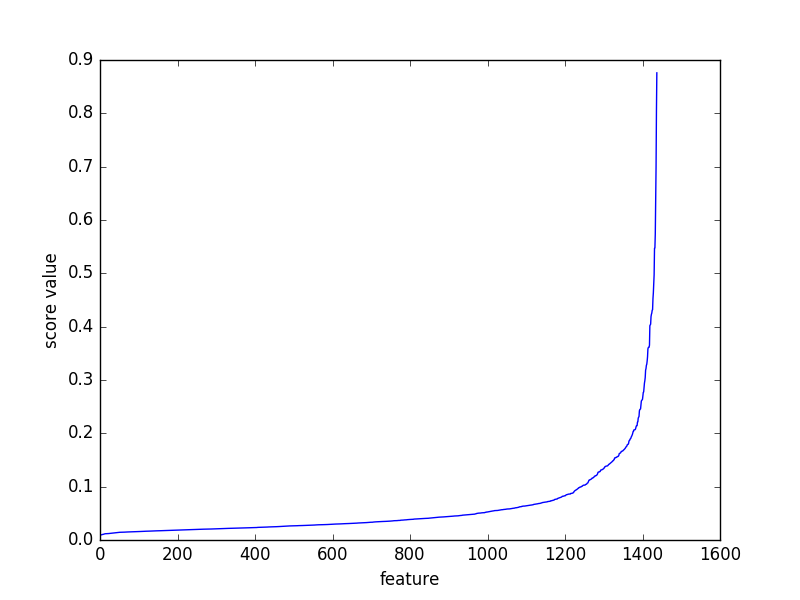
\includegraphics[width=0.5\linewidth]{pics/spec_unnorm_euclidean_no_first.png}
  \caption{График распределения признаков по важности. Слева базовый вариант, справа применение ядра}
  \label{kernel_blob}
\end{figure}

Как видно, применение ядер практически не влияет на значения важности признаков. Это связано с достаточно хорошей отделимостью кластеров в смоделированных данных. Стоит добавить применение ядра в алгоритм, чтобы сгладить шумовые эффекты.
\subsubsection{Регуляризация и неотрицательная факторизация матрицы признаков}
Такие алгоритмы как NDFS и UDFS для отбора признаков применяют неотризательную факторизацию матрицы признаков совместно с регуляризацией. Регуляризация позволяет эффективно обратить в 0 важность шумовых признаков.
\begin{figure}[h]
  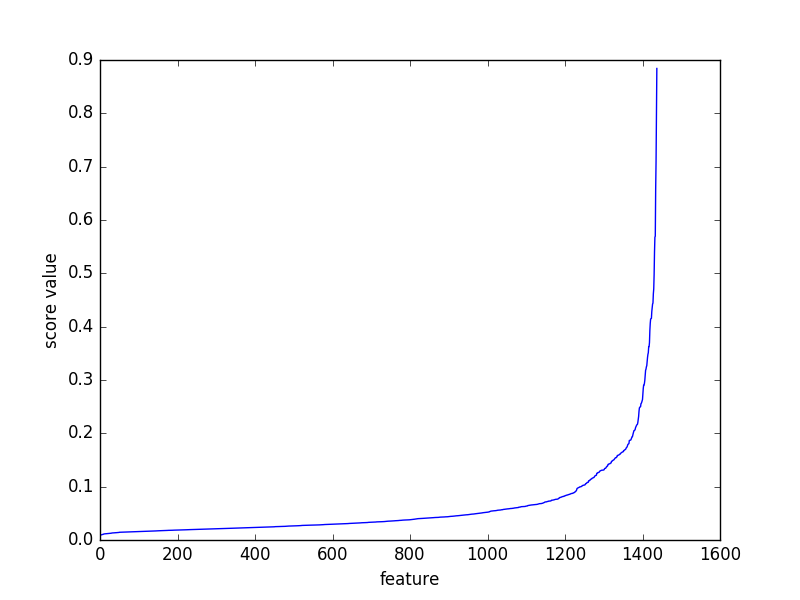
\includegraphics[width=0.5\linewidth]{pics/lp_unnorm_euclidean.png}
  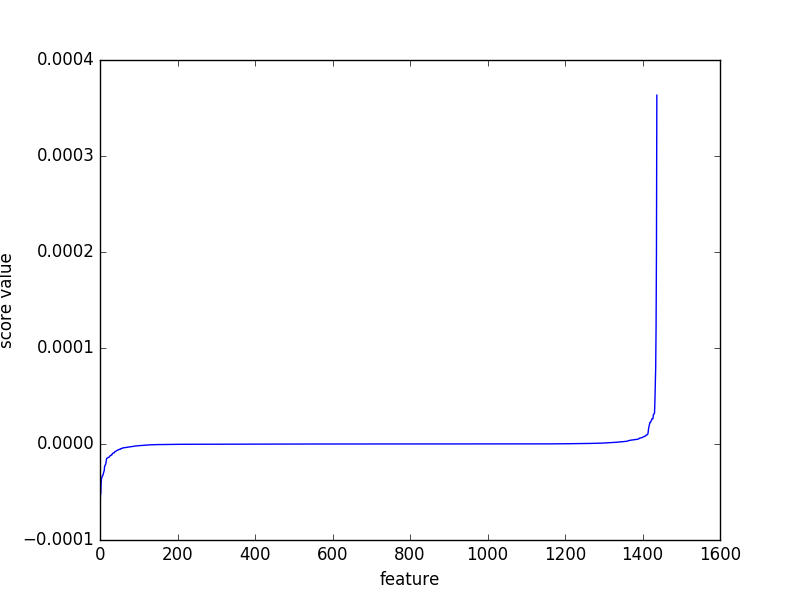
\includegraphics[width=0.5\linewidth]{pics/ndfs_unnorm_euclidean_3c.png}
  \caption{График распределения признаков по важности. Слева базовый вариант, справа применение регуляризации}
  \label{regularization_blob}
\end{figure}

Порог обращения в 0 можно установить, изменяя параметр регуляризации. 
\subsubsection{Отдельный отбор признаков для каждого кластера}
Алгоритм MCFS решает задачу оптимизации для каждого кластера. Полученное ранжирование признаков для каждого кластера затем нужно объединить в финальное ранжирование, усреднив или взяв максимум/минимум.

\begin{figure}[H]
  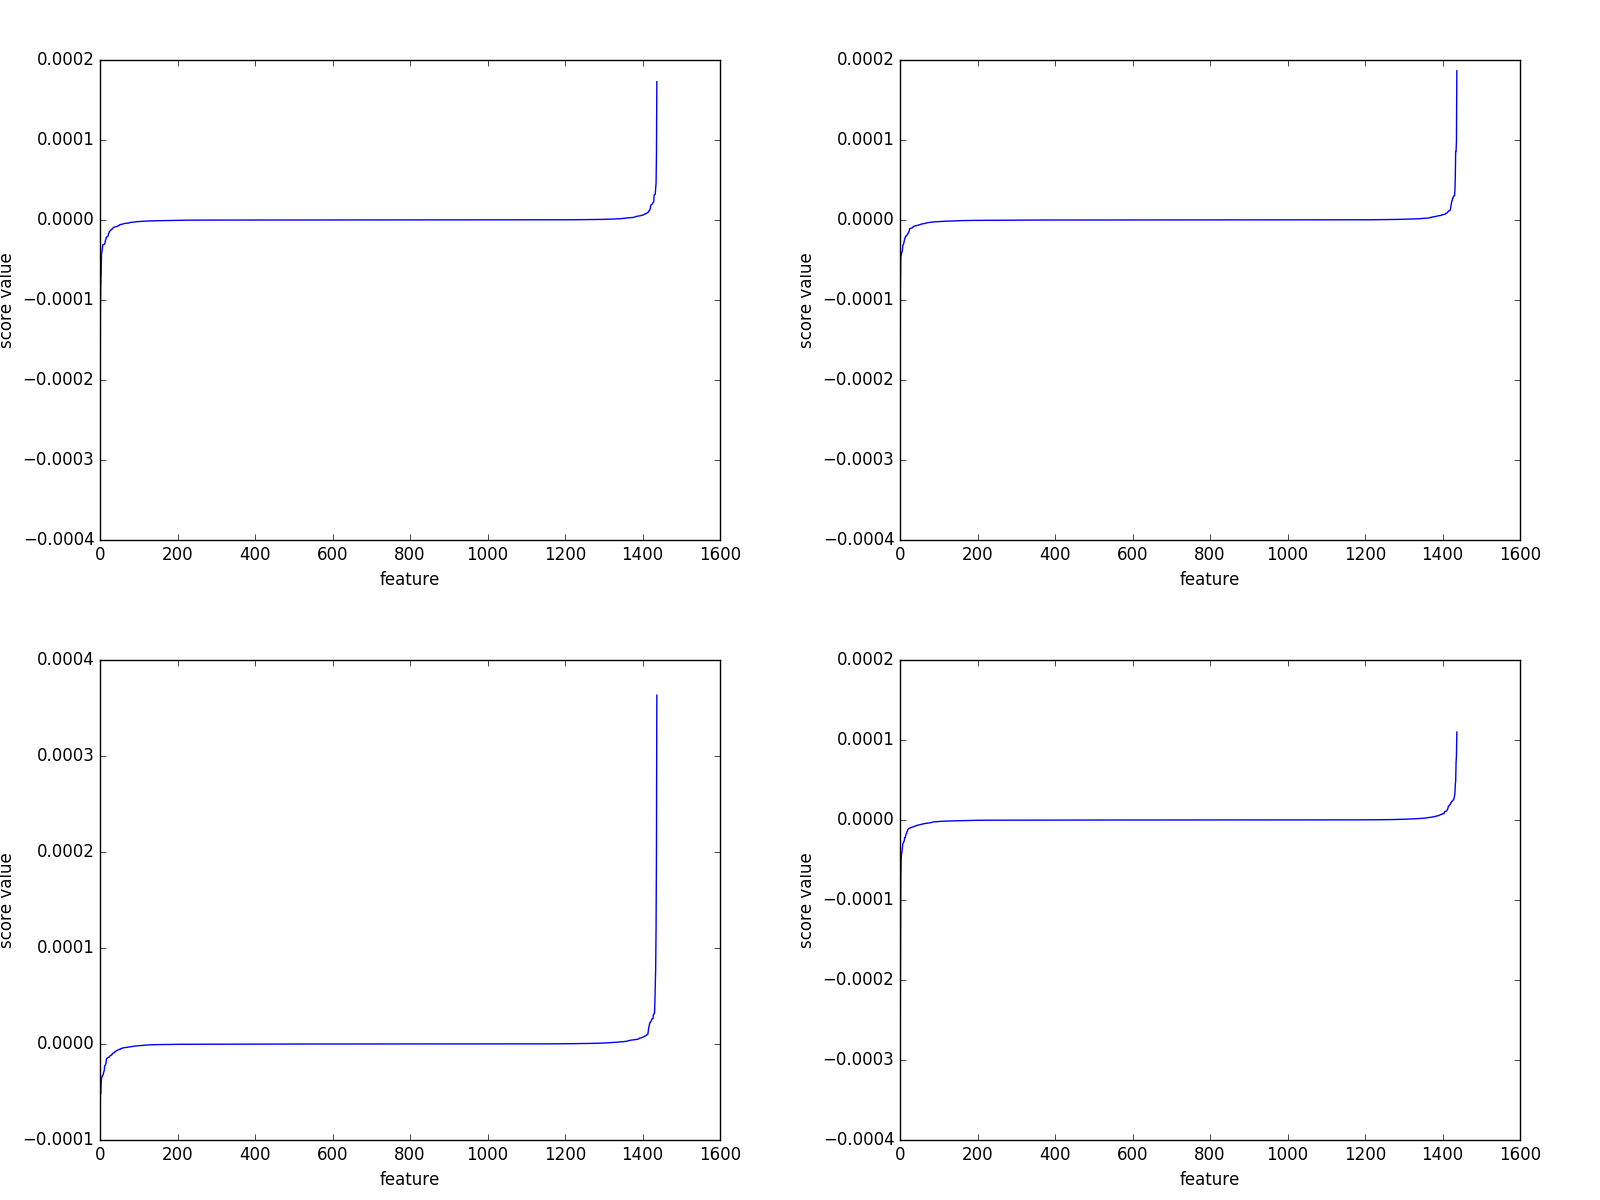
\includegraphics[width=\linewidth]{pics/ndfs_unnorm_euclidean.png}
  \caption{График распределения признаков по важности. Слева направо сверху вниз: кластеры 1,2,3,4}
  \label{regularization_blob}
\end{figure}
Видно, что значения показателя важности разделяются в каждом кластере. Подобное ранжирование поезно тем, что даёт информацию о характиристиках кластеров в исследуемых данных.
\subsubsection{Генетический алгоритм}
Для переформулировки задачи как задачи комбинаторной оптимизации, каждому возможному подмножеству признаков был поставлен в соответствие бинарный вектор $x \in \{0,1\}^n$, в котором 1 обозначает наличие признака в множестве, 0 -- отсутствие. Целевой функциуй было выбрана взаимная информация разбиения кластеризацией с оригинальными признаками и разбиения с отобранными признаками минус нормированное число взятых признаков. Максимум функции соответствует полному совпадению кластеризаций с минимальным количеством признаков. Размер популяции был выбран стандартный, 300 едини, скрещивание полное. Особенность мутации, вероятность перехода $0 \rightarrow 1$ значительно меньше, чем вероятность перехода $1 \rightarrow 0$,  что стимулирует отбрасывание признаков в каждом поколении.
\subsection{Основные результаты и выводы}
Был разработан окончательный вариант процесса кластеризации экзонов и отбора и ранжирования признаков, представленный на рисунке \ref{process}.
\begin{figure}[H]
\center
  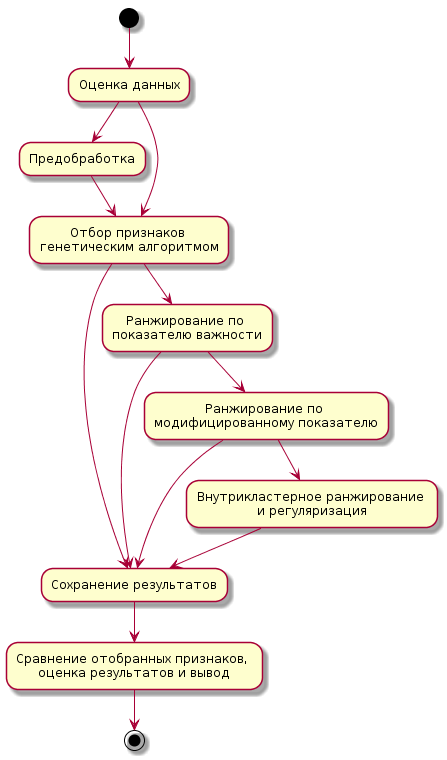
\includegraphics[width=0.5\linewidth]{pics/process.png}
  \caption{Процесс кластеризации и ранжирования важности признаков экзона}
  \label{process}
\end{figure}